% 原文 pp.21–28（印刷 pp.1139–1146）
% 第 1 讲（Lecture 1: Symmetry Breaking）第 3 部分：Goldstone 定理的证明与推论、
% 纯不可重整场论的红外行为（§1.7）、Goldstone 玻色子的有效作用量（§1.8）、参考文献

% ===== 原文 p.21 =====
于是 $\rho(m^2)=c\delta(m^2)$，其中 $c$ 是常数。常数 $c$ 不能为零，否则我们就会证明 $[J(x),\phi(0)]$ 在真空中的期望值为零，而这与对称性破缺的假设相矛盾。

这一论证表明，两点函数 $\langle\Omega,J(x)\phi(0)\Omega\rangle$ 的全部贡献都来自零质量的中间态。这意味着 $L^2(\mathcal{O}_0^+)$ 含于 $\mathcal{H}$ 的离散谱之中（即作为 Poincaré 群的一个真正的子表示（subrepresentation））。在场论中，这样的子表示被解释为一个自旋为零的无质量粒子。于是我们证明了下述命题，它就以 Goldstone 定理之名著称：

\noindent\textbf{定理}。\emph{在连续对称性破缺的场论实现所处的 Hilbert 空间 $\mathcal{H}$ 中，存在一个无质量标量（即 Poincaré 群的一个与 $L^2(\mathcal{O}_0^+)$ 同构的子表示），它由破缺对称性的流所产生。}

\noindent\textbf{注（Remark）}。「产生（created）」的意思是 $J(x)\Omega$ 与该子表示不正交。

\noindent\textbf{定义}。我们找到的这个无质量标量称为与破缺对称性 $G^s$ 相对应的 Goldstone 玻色子（Goldstone boson）。

\noindent\textbf{注 1}。若关于 $G^s$ 的对称性未被破缺，则 $\lim_{f\to1}Q_f\Omega$ 将为零。另一方面，当对称性破缺发生时，$Q_f$ 会从真空中产生 Goldstone 玻色子。因此，Goldstone 玻色子「度量」了对称性的失效。

\noindent\textbf{注 2}。Goldstone 玻色子不仅可由对称性的流算符产生，也可由其他局域算符产生。事实上，正如我们在 Goldstone 定理的证明中所见，任何一个标量局域算符，只要其单点函数在该对称性下不是不变的，它就会产生 Goldstone 玻色子。

\noindent\textbf{注 3}。Goldstone 定理并未断言 Goldstone 玻色子是自由的，即并未断言它可以由一个自由场 $\phi(x)$ 产生。事实上，正如我们将看到的，情况往往并非如此。

\noindent\textbf{注 4}。如果连续对称性破缺在经典层面就已发生，那么 Goldstone 玻色子在微扰论中已经可以看到。作为例子，考虑拉氏量 (1.13)。考虑经典基态 $\phi=a$。这个态是简并的。因此，如果我们引入实变量 $\phi_1=\operatorname{Re}\phi-a$，$\phi_2=\operatorname{Im}\phi$，并用这些变量改写拉氏量，那么由于极小值的简并性，场 $\phi_2$ 在经典上将是零质量的。因此，如果我们计算 $\phi_2$ 的两点函数，它将在 $k^2=0$ 处有一个极点（模掉微扰参数）。当然，在缺乏对称性的情况下，圈项可能移动这个极点。换句话说，经典上无质量的 $\phi_2$ 在量子层面可能获得非零质量。Goldstone 定理告诉我们的是：如果存在一个自发破缺的对称性，使得条件 $\phi_2=0$ 在该对称性下不是不变的，那么上述情形就不会发生。

% [Tutor Note: 注 4 中的「模掉微扰参数」有多层含义，易被读漏：其一，经典上 $\phi_2$ 的质量严格为零，是因为势沿 $U(1)$ 的轨道方向（即 $\phi_2$ 方向）是平坦的，二阶导数 $\partial^2V/\partial\phi_2^2|_{a}=0$ 是简并极小值的直接推论；其二，一旦计入圈图，$\phi_2$ 的自能会得到 $\mathcal{O}(\lambda)$ 的修正，从而把传播子的极点从 $k^2=0$ 移到 $k^2=\mathcal{O}(\lambda a^2)$；其三，作者说「若存在使 $\phi_2=0$ 不变性被破坏的自发破缺对称性，则极点仍钉在 $k^2=0$」，其实质是 Ward 恒等式（流守恒）把自能的极点位置与破缺生成元的单点函数绑定在一起。另须注意：本条只对 $d\ge3$ 成立；在 $d=2$ 时由本页推论，$\phi_2$ 不可能真正无质量（Coleman 定理），此时上面的微扰论证在红外区失效。]

\noindent\textbf{推论}。连续对称性破缺不会发生在 2 维中。

\noindent\textbf{证明}。否则，由 Goldstone 定理，Goldstone 玻色子就必须存在。但在二维量子场论中，不可能存在由局域算符产生的无质量粒子。的确，该算符在动量空间中的两点函数等于 $w(k^2)=\int_0^\infty\frac{d\mu(m^2)}{k^2+m^2}$，其中 $\mu$ 是谱测度（spectral measure）。如果

% ===== 原文 p.22 =====
存在无质量粒子，则该测度在 $m=0$ 处将有一个原子（atom，即 $\delta$ 型点质量）。但在此情形下，位置空间中的两点函数 $W(x)$ 在无穷远处将表现为 $-C\ln x^2$，也就是违反正性公理（positivity axiom）。$\square$

% [Tutor Note: 这里的「原子」是测度论的术语，指谱测度在 $m=0$ 处的点质量 $c\,\delta(m^2)$，而非物理上的原子；它正是上一页 $\rho(m^2)=c\delta(m^2)$ 中 $c\neq0$ 的另一种说法。$2$ 维无质量标量的 Wightman 函数在 Minkowski 号差下为 $\sim-\frac{1}{4\pi}\ln(-x^2+i0)$（Euclidean 中为 $-\frac{1}{2\pi}\ln|x|$），其对数的增长意味着它可以任意缓慢地发散，从而使某些检验函数的 smearing 给出负的「模方」，破坏 Hilbert 空间的正定性；系数的符号由 $|c|^2>0$ 固定，不能靠重新定义 $c$ 来翻转。严格的证明即 Coleman 定理（S. Coleman, Comm. Math. Phys. \textbf{31} (1973) 259），其论证依赖红外行为，与 $d\ge3$ 的情形有本质区别——高维时 $\ln$ 换成 $1/x^{(d-2)}$，衰减足够快，正性不受威胁。]

现在假设我们有一个具有李群 $G$ 对称性的拉氏量。假设 $\mathcal{H}$ 是由该拉氏量定义的量子场论的一个实现，其稳定化子（stabilizer）为 $H\subset G$。此时人们说：在实现 $\mathcal{H}$ 中，$G$ 对称性被自发破缺（spontaneously broken）到 $H$。（由上述推论，时空维数必然大于二。）

设 $\mathfrak{g},\mathfrak{h}$ 分别为 $G,H$ 的李代数。Goldstone 定理蕴涵

\noindent\textbf{推论}。$\mathcal{H}$ 的离散谱中含有一个与 $L^2(\mathcal{O}_0^+)\otimes(\mathfrak{g}/\mathfrak{h})$ 同构的子表示。

\noindent\textbf{证明}。证明是显然的：若非如此，则存在元素 $Y\in\mathfrak{g}$、$Y\notin\mathfrak{h}$，使得当 $f\to1$ 时 $Q_Y^f\Omega\to0$（弱收敛）。这意味着关于 $Y$ 的对称性未被破缺——矛盾。

% [Tutor Note: 「证明是显然的」省略了两步。第一步是：若 $Q_Y^f\Omega\to0$（弱），则由 $\Omega$ 在 $\mathcal{H}$ 上的循环性（cyclicity）可推出 $[Q_Y^f,A]\Omega\to0$ 对稠密多个局域算符 $A$ 成立，故 $Y$ 生成的单参数群在真空上平凡作用，即 $Y\in\mathfrak{h}$——这与 $Y\notin\mathfrak{h}$ 矛盾；这里用到 $\Omega$ 是分离态（separating），即 $A\Omega=0\Rightarrow A=0$。第二步是张量因子：$L^2(\mathcal{O}_0^+)\otimes(\mathfrak{g}/\mathfrak{h})$ 中 $\mathfrak{g}/\mathfrak{h}$ 是平凡表示，只贡献重数，故 Goldstone 玻色子的个数为 $\dim(\mathfrak{g}/\mathfrak{h})=\dim G-\dim H$（对紧致 $G$、闭子群 $H$）。注意商空间 $\mathfrak{g}/\mathfrak{h}$ 只在选定真空（即选定 $H$）后才有意义，换一个真空相当于把 $\mathfrak{h}$ 共轭化，重数不变但具体哪些生成元「破缺」会变。附带指出：原文 "if this is not so than there exists" 中的 than 应为 then，系原书排印笔误。]

该推论意味着：对应于线性无关的破缺无穷小对称性的 Goldstone 玻色子也是线性无关的。

\noindent\textbf{例}。设 $\phi:\mathbb{R}^d\to\mathbb{R}^N$ 是标量场，并考虑拉氏量

\begin{equation}
  \tag{1.30}
  \label{eq:1-30}
  \mathcal{L}(\phi)=\int d^dx\left(\frac12(\nabla\phi)^2+\frac{g}{4!}(\phi^2-a^2)^2\right).
\end{equation}

这个拉氏量具有 $SO(N)$ 对称性，其经典基态空间是 $S^{N-1}$。因此，经典上 $SO(N)$ 对称性被破缺到 $SO(N-1)$。如我们所知，若 $d>2$，同样的情形在量子层面也会发生（对于弱耦合理论），于是该理论的任何实现（解）都有 $N-1$ 个独立的 Goldstone 玻色子。

设 $P$ 是坐标为 $(0,0,\dots,0,a)$ 的经典极小点。考虑该理论的实现 $\mathcal{H}_P$，其中真空 $\Omega$ 局域化在 $P$ 附近。设 $Y_i\in\mathfrak{so}_N$，$i=1,\dots,N-1$，是 $\mathbb{R}^N$ 的基向量 $e_i,e_N$ 所生成的平面内的无穷小转动。算符 $\phi_i$ 的单点函数在 $Y_i$ 下不是不变的，因此 $\phi_i$ 产生对应于 $Y_i$ 的 Goldstone 玻色子。

我们可以构造低能（非真空）态，它们并非仅仅局域化在单个经典基态 $P$ 附近。的确，设 $P'$ 是另一个经典基态，并设 $Y\in\mathfrak{so}(N)$ 是使 $e^YP=P'$ 的元素。设 $J_Y$ 是对应于 $Y$ 的流，$Q_Y^f$ 是相应的截断电荷（cutoff charge）。则态 $e^{iQ_Y^f}\Omega$ 是一个局域化在 $P'$ 附近的低能态。

在长距离上，该理论的行为将如同一个映入经典基态空间的 $\sigma$ 模型。对 $N\ge3$ 这是一个有趣的论断，因为此时靶空间（$S^{N-1}$）不是平坦的，所以该 $\sigma$ 模型不是自由的。更确切地说，在低能（或长距离）下，玻色子 $\phi_i$（$i=1,\dots,N-1$）的理论在第零阶近似（即只考虑散射振幅的零动量极限）中是自由的，但在第一阶近似（即考虑小动量下的一阶非零项）中它将不再自由，而由映入球面的 $\sigma$ 模型的拉氏量描述。

% [Tutor Note: 此处 $Y_i$ 的选取有指标上的陷阱：$Y_i$ 是平面 $(e_i,e_N)$ 内的转动生成元，它把 $\phi_i$ 与 $\phi_N$ 混合，即 $\delta\phi_i\propto\phi_N$、$\delta\phi_N\propto-\phi_i$。在真空附近 $\phi_N\simeq a\neq0$ 而 $\langle\phi_i\rangle=0$，故 $\langle\delta\phi_i\rangle\propto a$ 不为零，$\phi_i$ 的单点函数确实破缺；反之若误取平面 $(e_i,e_j)$（$i,j<N$）内的转动，则 $\langle\delta\phi_i\rangle=0$，单点函数不变，那里的生成元属于 $\mathfrak{h}$，不产生 Goldstone 玻色子。这正好印证上一条推论：可用的破缺生成元恰为 $\dim(\mathfrak{so}_N/\mathfrak{so}_{N-1})=N-1$ 个。]

% ===== 原文 p.23 =====
\subsection{纯不可重整场论的红外行为}
% 原文 §1.7：Infrared behavior of purely non-renormalizable field theories

在本节中，我们将澄清下述论断的含义与依据：对于 $d>2$，一个所有无质量粒子都是 Goldstone 玻色子的量子场论，在红外极限下的行为如同一个映入真空态空间的 $\sigma$ 模型。

假设我们有一个由拉氏量 $\mathcal{L}$ 描述的纯不可重整（purely nonrenormalizable）场论。若一个拉氏量的所有耦合都具有负的标度维数，我们就称它为纯不可重整的。这类拉氏量的一个例子是 $d>2$ 的 $\sigma$ 模型的拉氏量。这样的拉氏量不适合在 UV 极限下做微扰重整化，但在 IR 极限下不造成任何问题，因为从 Wilson 重整化群流的观点看，它们的所有相互作用都是 IR 无关（irrelevant）的。也就是说，如果我们引入一个 UV 动量截断 $\Lambda$（此时并不将它送到无穷），就可以微扰地定义 $\mathcal{L}$ 的关联函数：关联函数是所有费曼图振幅之和，这些图按通常方式计算，积分在 $|q|<\Lambda$ 处截断。由于 $\mathcal{L}$ 没有质量项，可能存在一些 IR 发散，但当所有耦合都具有负维数时，它们是相当温和的；它们的含义只是：$S$ 矩阵在零动量附近的动量中不是解析的。（我们稍后会给出一个例子；参看本讲末尾的那张图。）

现在假设我们想计算动量表象中 $n$ 点函数在点 $k_i=0$ 附近的渐近展开。我们将有（其中 $\sum k_i=0$）：

\begin{equation}
  \tag{1.31}
  \label{eq:1-31}
  G_n(k_1,\dots,k_n)=\frac{G_n^0(k_1,\dots,k_n)}{k_1^2\cdots k_n^2},
\end{equation}

其中，按照我们在 Kazhdan 的讲演中学到的 LSZ 约化公式，$G_n^0$ 是 $n$ 个 Goldstone 玻色子散射的 $S$ 矩阵元。$G_n^0$ 在 $k_i=0$ 附近不是解析的，因此我们不能把它展开成幂级数；但我们可以考察它在整体标度变换 $k_i\to\lambda k_i$ 下的行为。

这个级数的关键性质（它来自纯不可重整性）是：模掉按 $\lambda$ 的任意给定幂次标度的项，$G_n^0$ 由有限多个费曼图决定。换句话说，纯不可重整性加上量纲分析蕴涵：越来越高阶的项按 $\lambda$ 的越来越高次幂标度。因此，我们只须借助微扰论中有限多项，就能得到关联函数在 $k_i$ 中任意阶的 IR 渐近行为。

% [Tutor Note: (1.31) 只是把「去掉外腿传播子」这一步写成了公式，切勿把 $G_n^0$ 与 $n$ 点 Green 函数 $G_n$ 混为一谈：$G_n$ 在每个 $k_i^2\to0$ 处有极点（极点留数即 $S$ 矩阵元），故 $G_n$ 本身根本没有 $k_i\to0$ 的幂级数展开，只有去掉极点因子后的 $G_n^0$ 才有。所谓「按 $\lambda$ 的幂次标度」，指的是在 $k_i\to\lambda k_i$ 下令 $\lambda\to0$：$G_n^0$ 的展开中第 $m$ 阶项恰含 $2m$ 个导数，故按 $\lambda^{2m}$ 标度（等价地，每个额外导数贡献一个 $\lambda$ 的幂）。若自行推导，注意 $n$ 个外腿的极点因子共给出 $\lambda^{2n}$，并且不同作者对外腿的归一化（是否提出整体常数、是否用 $\mathrm{i}$ 因子）约定不同，比较结果前须先核对这一点。]

在纯不可重整理论中构造的圈图当然也有紫外发散。我们把该纯不可重整理论视为低能有效场论，从这个观点看，我们只是以任意方式正规化这些发散，并把低能有效拉氏量中所有可能项的系数当作唯象参数。模掉 $\lambda$ 的任意幂次，只有有限多个这样的项是相关（relevant）的（因为当 $d>2$ 时，只有有限多个维数低于某个给定常数的算符）。

现在假设我们有一个真正的量子场论，由某个可重整拉氏量 $\mathcal{L}'$ 给出。当我们说由 $\mathcal{L}'$ 定义的理论在 IR 极限下、在给定精度内由（同一组场上的）纯不可重整拉氏量 $\mathcal{L}$ 描述时，我们的意思是：模掉在 $k_i\to\lambda k_i$ 下按 $\lambda$ 的给定幂次标度的项，由 (1.31) 给出的函数 $G_n^0$ 对 $\mathcal{L}$ 与对 $\mathcal{L}'$ 是相同的。

% ===== 原文 p.24 =====
例如，当我们在上一节末尾说，在低能（或长距离）下，玻色子 $\phi_i$（$i=1,\dots,N-1$）的理论在第零阶近似中是自由的，而在第一阶近似中由坐标为 $\phi_i$ 的球面上的 $\sigma$ 模型的拉氏量描述时，我们的意思是：$\phi_i$ 的函数 $G_n^0(k_1,\dots,k_n)$ 与自由理论中的相同（模 $o(1)$），并与 $\sigma$ 模型中的相同（模 $o(k^2)$）。

计算 $k$ 展开的更高阶项，人们可以构造一个纯不可重整的低能有效理论，它将在红外区以任意所需的精度描述我们的理论。

\noindent\textbf{注}。由于函数 $G_n^0(k_1,\dots,k_n)$ 到轨迹（locus）$k_i^2=0$（其中 $k_i$ 不必为零）上的限制就是 $S$ 矩阵元，该断言的意思是：在 $k^0$ 阶，模型 (1.30) 中 $n$ 个 Goldstone 玻色子的散射矩阵与自由理论中一样为零；而 $k^2$ 阶的项由真空态空间的曲率决定，特别地当 $N>2$ 时不为零。

\subsection{Goldstone 玻色子的有效作用量}
% 原文 §1.8：Effective action for Goldstone bosons

让我们落实上一节的一般讨论，并在一个具体例子中算出 Goldstone 玻色子的有效作用量（effective action）。考虑一个把 $SO(3)$ 破缺到 $SO(2)=U(1)$ 的理论。我们有三个实标量，它们可以组合成一个三分量对象 $\vec\phi$，在 $SO(3)$ 的三维表示中变换。拉氏量为

\[
  \mathcal{L}=\frac1\lambda\int d^nx\left[\frac12(\partial_\mu\vec\phi)^2+V(|\vec\phi|)\right],
\]

其中，令 $\rho=|\vec\phi|$，$V(\rho)$ 是一个在原点之外具有非退化极小值的势。

\begin{figure}[htbp]
  \centering
  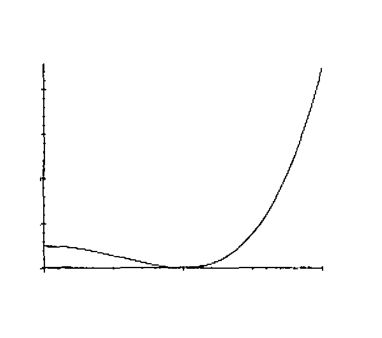
\includegraphics[width=0.40\textwidth]{figs/fig_p024_1.png}
  \caption{势 $V(\rho)$ 的形状：曲线在 $\rho=\rho_0>0$ 处达到极小并触及横轴，向左（$\rho\to0$）略微回升，向右则陡升；纵轴带有分度刻线，原图未标注坐标轴名称与数值。（原文 Figure 1，p.24）}
  \label{fig:p24-1}
\end{figure}

最简单的这类势是 $V(\rho)=\frac18(\rho^2-\rho_0^2)^2$，其极小值在 $\rho_0$ 处。若令 $\Omega=\phi/\rho\in S^2$，我们可以把拉氏量改写为

\[
  \mathcal{L}=\frac1\lambda\int d^nx\Bigl[
  \frac12(\partial_\mu\rho)^2
  +\frac12\rho^2(\partial_\mu\Omega)^2
  +V(\rho)\Bigr].
\]

项 $\frac12\rho^2(\partial_\mu\Omega)^2$ 代表 $S^2$ 上的圆度规（round metric）。

当 $\lambda$ 很小时，我们可以期望经典近似是好的。由于 $\rho$ 是有质量的场，我们可以把它从理论中积掉：令它等于其极小值 $\rho_0$，并研究涨落

\[
  \rho=\rho_0+w,
\]

其中 $w$ 现在是出现在我们路径积分中的量子场。到第一阶近似，我们将有有效拉氏量

\[
  \mathcal{L}_{\mathrm{eff}}(\Omega)=\frac{\rho_0^2}{2\lambda}\int d^nx\,(\partial\Omega)^2,
\]

% [Tutor Note: 由 $\Omega=\phi/\rho$ 到 $\frac12\rho^2(\partial_\mu\Omega)^2$ 这一步用到了 $|\Omega|^2=1$ 的约束：把 $\vec\phi=\rho\,\Omega$ 代入 $\frac12(\partial_\mu\vec\phi)^2$，得 $\frac12(\partial_\mu\rho)^2+\rho\,\partial_\mu\rho\,\Omega\cdot\partial_\mu\Omega+\frac12\rho^2(\partial_\mu\Omega)^2$，其中交叉项因 $0=\partial_\mu(\Omega^2)=2\Omega\cdot\partial_\mu\Omega$ 而消失——这个消去是关键，漏掉它就会多出一个 $\rho\,\partial_\mu\rho\,\Omega\cdot\partial_\mu\Omega$ 型的项。另外注意 $\Omega$ 取值于 $S^2$，故 $(\partial_\mu\Omega)^2$ 必须理解为由 $S^2$ 的圆度规缩并：$g_{ij}(\Omega)\partial_\mu\Omega^i\partial_\mu\Omega^j$，这正是「$\frac12\rho^2$ 是度规的共形因子」一语的含义。]

% ===== 原文 p.25 =====
它描述一个映入 $G/H$ 的非线性 $\sigma$ 模型，在目前情形下 $G/H$ 就是 $S^2$。无质量场由 $\Omega$ 描述。

这能是答案吗？换句话说，是否任何量子场论都能在红外区流向这个 $\sigma$ 模型？事实上，对于时空维数 $n>2$，它确实是一个可能的答案，因为非线性 $\sigma$ 模型在二维以上是不可重整的，所以我们得到的相互作用是无关的。也就是说，若 $a_i$ 是 $S^2$ 上点 $P$ 附近的 Riemann 法坐标（Riemann normal coordinates），我们可以在 $P$ 附近示意地展开

\[
  (\partial\Omega)^2=(da)^2+R\,a^2(da)^2+\cdots
\]

其中 $R$ 是 $S^2$ 的 Riemann 张量。由此我们看到该相互作用在二维以上是无关的。事实上，为给 $(da)^2$ 以维数 $n$，我们必须赋予 $a$ 以维数 $(n-2)/2$，于是该相互作用的维数为 $2n-2$，当 $n>2$ 时超过 $n$。$\sigma$ 模型对 $n>2$ 是可能的答案而对 $n\le2$ 不是，这一点是前面讨论过的事实的另一个侧面：连续对称性的自发破缺对 $n>2$ 可能、对 $n\le2$ 不可能。这一展开也可以作为从 $\sigma$ 模型显式计算 Goldstone 玻色子 $S$ 矩阵的出发点。

% [Tutor Note: 这个展开写得很「示意」，严格的形式是：在法坐标下 $S^2$ 的度规为 $g_{ij}(a)=\delta_{ij}-\frac13R_{ikjl}a^ka^l+O(a^3)$，于是 $(\partial_\mu\Omega)^2=g_{ij}(a)\partial_\mu a^i\partial_\mu a^j=(da)^2-\frac13R_{ikjl}a^ka^l\partial_\mu a^i\partial_\mu a^j+\cdots$；原文把它压缩成 $R\,a^2(da)^2$，其中 $R$ 泛指 Riemann 张量（在 $S^2$ 这一二维情形它只有一个独立分量，正比于曲率标量），系数 $\frac13$ 与四个指标的具体缩并方式被吸收进「$\cdots$」。做量纲计数时还要注意 $(da)^2$ 是 $(\partial_\mu a)^2$ 的缩写（$[\partial_\mu]=1$），故 $[a]=(n-2)/2$，而 $R\,a^2(da)^2$ 的维数为 $-2+2\cdot\frac{n-2}{2}+n=2n-2$，与原文结论一致。]

$\sigma$ 模型是否是我们这个具体问题红外行为的正确答案（至少对足够小的 $\lambda$）？我们断言是的。为研究这一点，让我们微扰地处理 $w$ 的效应。$w$ 与 Goldstone 玻色子的相互作用来自拉氏量中的相互作用项：

\[
\begin{aligned}
  \frac1{2\lambda}\rho^2(\partial\Omega)^2
  &=\frac1{2\lambda}(\rho_0+w)^2(\partial\Omega)^2\\
  &=\frac1{2\lambda}(\rho_0^2+2\rho_0w+w^2)(\partial\Omega)^2.
\end{aligned}
\]

算符 $\partial\Omega$ 是高度非线性的，可以认为它能发射任意多个 Goldstone 玻色子。为了求出有效拉氏量，我们需要计算涉及 $w$ 的费曼图。一个典型的图是

\begin{figure}[htbp]
  \centering
  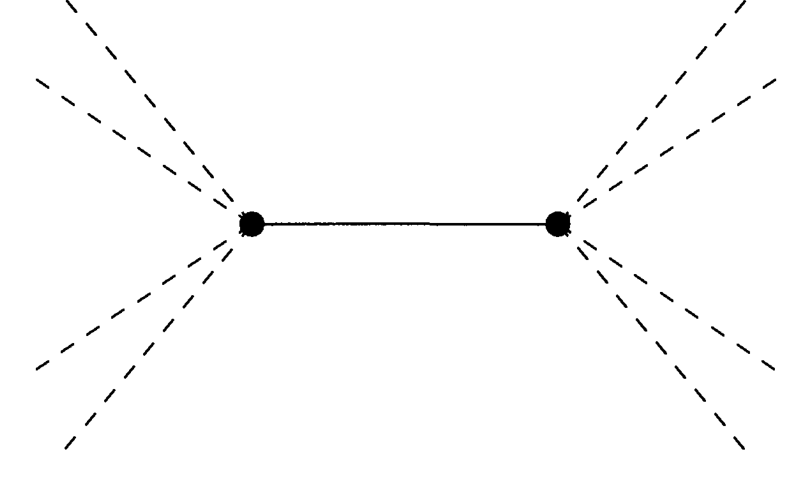
\includegraphics[width=0.60\textwidth]{figs/fig_p025_1.png}
  \caption{$w$ 场的交换图：实线代表有质量的 $w$ 场，虚线代表 $a$（即 $\Omega$ 的涨落，也就是 Goldstone 玻色子）；两个黑点表示来自 $\rho^2(\partial\Omega)^2$ 的顶点，每个顶点各连出四条外线（虚线的多重性来自 $(\partial\Omega)^2$ 的任意阶展开）。（原文 Figure 1，p.25）}
  \label{fig:p25-1}
\end{figure}

这里我们用实线表示 $w$，用虚线表示 $a$。$w$ 的传播子是 $\frac1{k^2+m_w^2}$；由于我们关心小动量 $k$，我们按 $k$ 的幂次展开。领头项是

\[
  \mathrm{const}\cdot(\partial\Omega)^2\frac1{m_w^2}(\partial\Omega)^2.
\]

它具有 $SO(3)$ 对称性，而且是一个无关的相互作用。它甚至比上面草绘的那些来自把 $(\partial\Omega)^2$ 按 $a$ 的幂次展开的项更加无关。

事实上，尽管研究这些图很有教益（哪怕只是为了说明 $\sigma$ 模型是红外稳定的），我们并不需要图的细节。我们所需要知道的只是：有效作用量具有 $SO(3)$ 对称性。给定这一对称性，有效作用量中可能产生哪些项呢？

% ===== 原文 p.26 =====
\begin{itemize}
\item 势 $V(\Omega)$ 不可能出现，因为 $S^2$ 上不存在 $SO(3)$ 不变的函数。这正是给定 $SO(3)$ 对称性后 $\sigma$ 模型红外稳定的基本原因。一个势函数会完全改变图景。例如，一个一般的势会有一个孤立的、非退化的极小值，从而给我们一个唯一的真空以及一个红外平庸的有质量理论，这与自发破缺的 $SO(3)$ 所联系的连续真空族形成对照。
\item 唯一只含两个导数、且尊重问题全部对称性的项就是 $(\partial\Omega)^2$ 本身。（这本质上是因为 $S^2$ 上任何 $SO(3)$ 不变的度规都是标准度规的倍数。）因此，理所当然应当预期：由含 $w$ 场的图带来的量子修正会改变这一项的系数。
\item 其他可能的项，如 $(\partial\Omega^2)^2$ 与 $(\partial\Omega)\nabla^2(\partial\Omega)$，含有多于两个的导数，因而越来越无关。
\end{itemize}

于是，领头的红外行为由形如 $\frac1{f^2}(\partial\Omega)^2$ 的有效作用量决定，其中

\[
  \frac1{f^2}=\frac{\rho_0^2}{2\lambda}+\text{圈修正}.
\]

% [Tutor Note: 上列第三条中的 $(\partial\Omega^2)^2$ 应读作 $((\partial\Omega)^2)^2$：本节末尾讨论 $k^4$ 阶新常数时，作者自己写的就是 $((\partial\Omega)^2)^2$，可见这里是原书排印时少了一层括号（若照字面读成 $(\partial_\mu\Omega^2)^2$，指标根本无从缩并）。同理 $(\partial\Omega)\nabla^2(\partial\Omega)$ 的严格写法是 $\partial_\mu\Omega\,\nabla^2\partial_\mu\Omega$，其中 $\nabla^2=\partial_\nu\partial_\nu$ 作用在第二个因子上。另注意 $f$ 的归一化：此处 $\Omega$ 是无量纲的 $S^2$ 坐标、作用量写作 $\frac1{f^2}(\partial\Omega)^2$，与把 $\pi$ 介子场写成 $\Omega=\exp(2i\pi^a\tau^a/f_\pi)$ 的常见约定相差一个常数因子，故 $f$ 并非通常的衰变常数 $f_\pi$；跨文献比较数值前必须先统一 $\Omega$ 的归一化。]

把这个作用量在某个给定真空（即给定点 $P\in G/H$）附近的 Riemann 法坐标中展开时，就得到涉及 $G/H$ 的 Riemann 张量及其协变导数的相互作用（其中第一个已在上面草绘）。如果用这些相互作用计算涉及小动量（量级为 $k$）的 Goldstone 玻色子的散射振幅，则在 $k$ 接近零时，树图振幅全都正比于 $k^2$，因为相互作用项都恰好含有两个导数。当 $k\to0$ 时圈贡献更小，因为这些相互作用在红外区是无关的。更确切地说，圈图振幅要么 (i) 重整化 $SO(3)$ 不变拉氏量中的常数 $f$，要么 (ii) 给出在 $k\to0$ 时比 $k^2$ 更快趋于零的散射振幅修正。

因此，Goldstone 玻色子散射中 $k^2$ 阶的各项完全由单个常数 $f$ 决定（更一般地说，由齐性空间（homogeneous space）$G/H$ 上一个 $G$ 不变度规的选取决定）。1960 年代人们发现，$\pi$ 介子的低能散射漂亮地符合这样的描述，其中 $G=SU(2)\times SU(2)$，$H$ 是对角的 $SU(2)$。强相互作用具有自发破缺的近似手征对称性（chiral symmetry），就是以这种方式被发现的；这一发现对此后物理学的发展起了非常重要的作用。

如果人们想计算 Goldstone 玻色子散射中比 $k^2$ 更高阶的项，会怎样？显然，在 $k^4$ 阶会有新的常数进入，它们只能由微观计算（或实验）确定，因为存在含四个导数的 $G$ 不变相互作用（例如上面由所考虑的显式树图得到的 $((\partial\Omega)^2)^2$ 项）。然而有趣的是，在四维时空中，Goldstone 玻色子 $k^2$ 振幅的最低阶修正不是 $k^4$ 阶，而是 $k^4\ln k$ 阶。它来自一个圈图，

% ===== 原文 p.27 =====
\begin{figure}[htbp]
  \centering
  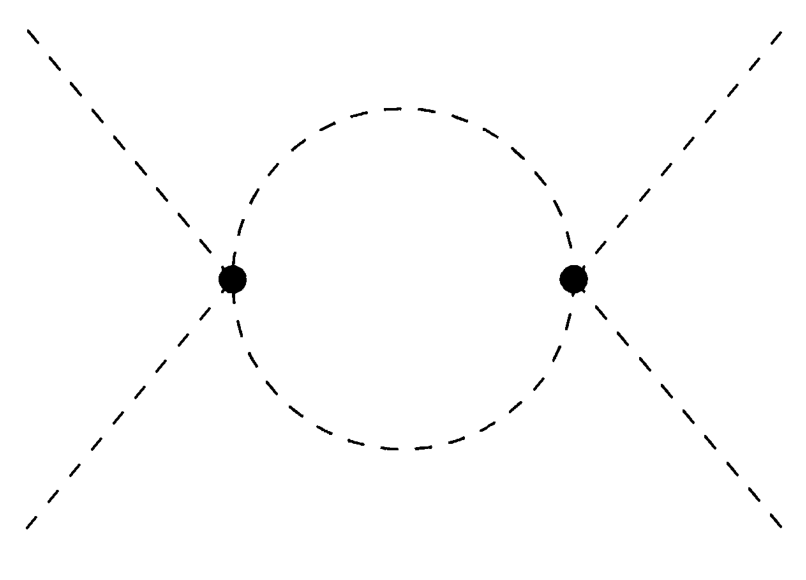
\includegraphics[width=0.56\textwidth]{figs/fig_p027_1.png}
  \caption{给出 $k^4\ln k$ 修正的单圈图：两个顶点取自拉氏量中含两个导数的部分，两个顶点各连出两条外线（虚线），二者之间由两条虚线连成圈（$a$ 场即 Goldstone 玻色子）。（原文 Figure 1，p.27）}
  \label{fig:p27-1}
\end{figure}

其顶点取自拉氏量的两导数部分，因此它完全由控制散射振幅中 $k^2$ 项的那个同一常数 $f$ 唯一确定。

% [Tutor Note: 「$k^4\ln k$ 而非 $k^4$」是量纲分析容易漏掉的一步：树图只有两个导数，故振幅 $\sim k^2$；四导数树图给出 $k^4$，系数是新的自由常数；而这个单圈图的两个顶点各含两个导数，共四个导数，按幂次计数本应为 $k^4$，但在 $d=4$ 时圈积分 $\int d^4q\,\frac{1}{q^2}\frac{1}{(q+k)^2}$ 是临界的，出现 $1/\varepsilon$ 极点，抵消极点后剩下的就是 $\ln k$（红外端由外动量 $k$ 截断），于是量纲上「应该」是 $k^4$ 的项被 $\ln k$ 修饰。这类项被称为手征对数（chiral log）：它的系数不含任何新参数，完全由 $f$ 与 $G/H$ 的曲率固定——这正是低能定理的威力所在，也是流代数能做出可检验预言的原因。]

通过我上面解释的想法对低能 Goldstone 玻色子相互作用所作的分析，被称为「流代数（current algebra）」。特别地，借助流代数关系，人们可以从实验推断破缺对称群 $G$ 是什么，以及 $G$ 不变有效拉氏量中的许多参数。

关于诸如本例这样的对称性破缺例子，最后一点评论：如果我们从一个 $G$ 不变的微观拉氏量 $\mathcal{L}_{\mathrm{micro}}$ 出发，并将其微扰为

\[
  \mathcal{L}_{\mathrm{micro}}+\varepsilon(\delta\mathcal{L}),
\]

其中 $\varepsilon$ 是小参数，且 $\delta\mathcal{L}$ 这一项不是 $G$ 不变的，那么在红外区我们将得到

\[
  \frac1{f^2}(\partial\Omega)^2+\varepsilon V(\Omega)+O(\varepsilon^2),
\]

其中 $V(\Omega)$ 是一个非 $G$ 不变的算符——它最重要的部分当然是不含导数的势，正如记号 $V$ 所提示的。$V(\Omega)$ 受到高度约束，因为它在 $G$ 下必须与 $\delta\mathcal{L}$ 以同样的方式变换。例如，在强相互作用的情形中，确实存在一个小的 $\delta\mathcal{L}$ 项，它把 $SU(2)\times SU(2)$ 破缺到对角 $SU(2)$；它从原本会是连续族的真空中选出一个唯一真空，并给 $\pi$ 介子以小的质量。（关于这一点，详见习题课中的问题 1。）由于 $\pi$ 介子实际上有质量，人们不能把它的四维动量展开到零附近；在 $\pi$ 介子的流代数研究中，实际上取动量 $k$ 为 $\pi$ 介子质量的量级。

\subsection*{参考文献与交叉引用}

关于场论的一般性，特别是对称性这一概念，更多内容见 [I-Classical Fields]（经典）与 [I-Axiomatics]（量子）。§§1.1、1.2 的非微扰估计是瞬子计算的例子，第 7 讲对之讨论得更详细。二维中角值自由场的理论在 [II-CFT] 的第 1 讲以及本系列的第 6 讲中讨论。关于 Goldstone 玻色子是四维中唯一自旋为 $0$ 的无质量粒子的讨论见第 2 讲。场论红外行为的一般性讨论见第 2 讲，后面各讲中有大量例子。这些讲末尾的问题 1 涉及对称性破缺。

% [Tutor Note: [I-Classical Fields]、[I-Axiomatics]、[II-CFT] 是本丛书（\emph{Quantum Fields and Strings: A Course for Mathematicians}）第 I、II 卷中对应章节的代号：I 卷讲经典场论与公理化场论，II 卷含共形场论（CFT）部分；作者用它们代替具体的页数引用。此处「二维中角值自由场」指取值于 $S^1$ 的自由标量场，其顶点算符 $e^{in\varphi(x)}$ 的关联函数按幂律衰减、标度维数与 $n^2$ 成正比，是二维 CFT 的基本构造块，与本讲讨论的 Goldstone 玻色子（取值于 $G/H$ 的非线性 $\sigma$ 模型）在二维的失效密切相关。]

关于二维时空中不存在自发对称性破缺的 Coleman 定理，可见

\begin{quote}
S. Coleman, \emph{There Are No Goldstone Bosons In Two Dimensions}, Commun. Math. Phys. \textbf{31} (1973), 259.
\end{quote}

% ===== 原文 p.28 =====
关于自发破缺的整体对称性及其蕴涵的入门介绍，见

\begin{quote}
S. Coleman, \emph{Aspects Of Symmetry}, Cambridge University Press, 1985.\\
S. Weinberg, \emph{The Quantum Theory Of Fields}, chapter 19, vol. 2, Cambridge University Press, 1996.
\end{quote}
